\subsubsection{Text Analyzing}

In this project, the chatbot will just have to identify the subjects and terms the students wish to know about and if any knowledge about it exists in the database. This can be done by identifying nouns and seeing if there is a match to any existing data in the database.
POS tagging will be used to pick out a part of a sentence by finding the first and last noun, together with the first and last adjective and looking at everything in between, seeing as how all subjects the chatbot has to know about will be described using verbs or adjectives. The chatbot will then check both the part of the sentence it has picked out as a whole, along with the individual nouns and adjectives, and see if they match with any of the subjects or terms known by the chatbot. \Figureref{fig:NLP_example2} shows a part of speech tagging example of the sentence "what are functions and numbers" a sentence which a student realistically could give the chatbot. The brackets show which part of the sentence the chatbot would pick out and try to find some knowledge about.

\begin{figure}[H]
    \centering
    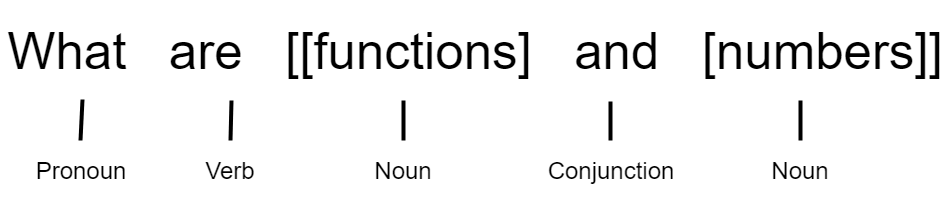
\includegraphics[width=0.6\textwidth]{figures/NLP_example2.png}
    \caption{Example of part of speech tagging}
    \label{fig:NLP_example2}
\end{figure}

\noindent
The chatbot will then check the database for knowledge on functions and numbers both as part of the same subject and individually, and if it exists present the knowledge to the user.

\begin{algorithm}[H]
    \begin{algorithmic}[1]
        \fontsize{7}{10}
        \fontencoding{T1}\ttfamily
        \Function{Analyze}{$WL$}
        \Statex \(\triangleright\) \textit{WL = The list of words to analyze}
        
        \textsc{WL.}\textproc{WordlistToText}\textsc{()}
        
        \If{\textsc{WL == command}}
            \textproc{DoCommand()}
        \EndIf
        
        \If{\textsc{No nouns}}
            \textproc{return "I did not understand"}
        \EndIf
        
        
        \textproc{FirstIndex = GetTheFirstIndexOfTheFirstNounOrAdjective(WL)}
        \textproc{LastIndex = GetTheLastIndexOfTheFirstNounOrAdjective(WL)}
        
        \textproc{Range = AllWordsBetweenFirstAndLastIndex(FirstIndex, LastIndex, WL)}
        
        \If{\textsc{If adjectives in Range are followed by something else than another adjective or a noun}}
            \textproc{return "Please write a proper sentence"}
        \EndIf
        
        \If{\textsc{If 2 commas are followed by each other}}
        \textproc{return "Please write a proper sentence"}
        \EndIf
        
        \If{\textsc{If WL contains any "," or "and" and the last of the 2 is not "and"}}
        \textproc{return "Please write a proper sentence"}
        \EndIf
        
        
        \EndFunction
    \end{algorithmic}
    \caption{Pseudo code of processing sentences}
    \label{alg:gruppering_af_blokke}
\end{algorithm}